\section{Benchmarking Various Unstructured Grid Implementations}	\label{sec:results}

In this section we compare the run times of several benchmarks on unstructured and regular grids on three real-world stencils. By applying the same set of stencils on both regular and unstructured grids, we show the effectiveness of the various previously described strategies for grid access and grid storage (see sections \ref{sec:grid-implementations}, \ref{sec:optimizations}). Furthermore, we use key metrics that are made available through the Nvidia profiler in order to better understand what causes the differences in performance.

Real-world stencil applications are applied in a multitude of different scenarios which result in differing problem domain sizes, precision requirements and properties of the stencils themselves. In combination with the different grid access and storage methods described in this report, this leads to a large number of potential setups to be tested. The benchmarks we executed can be characterized by the following properties:

\begin{itemize}
	\item 
		Input/output conditions 
		\begin{itemize}
			\item Domain size (size of the input and output grids)
			\item Required precision (single or double precision)
		\end{itemize}
	\item
		Stencil properties
		\begin{itemize}
			\item \emph{Arithmetic intensity:} The computational effort required to perform the actual output calculations given all input fields
			\item \emph{Number of input and output fields:} How many different values each cell in the grid contains and the stencil operates on
			\item \emph{Depth and number of neighborship dependencies}
		\end{itemize}
	\item
		\emph{Kernel launch configuration:} number of threads, blocks and bytes of shared memory
	\item
		Grid storage implementation properties
		\begin{itemize}
			\item Memory layout and potential regular patterns of stored values
			\item 
				Memory layout of neighborship storage
				\begin{itemize}
					\item Depth of stored neighbor pointers (pointer chasing)
					\item Compression of neighborship table
				\end{itemize}
		\end{itemize}
	\item
		Used grid access implementations
\end{itemize}

In the following, an overview of the benchmark results for the different possible combinations of these properties are given.

\subsection{Benchmarked Stencils and General Benchmark Setup}\label{sec:benchmark-setup}

We benchmark three stencils called \emph{laplace of laplace} (\emph{laplap} for short), \emph{horizontal diffusion} (\emph{hdiff} for short) and \emph{fast waves}. These stencils represent real-world use cases in meteorology applications. Table \ref{tab:benchmarked-stencils} details the values of the main stencil characteristics as listed in the bullet list above.

The definitions of all three stencils are given in terms of a regular grid. Thus, to measure the overhead of using an unstructured grid with indirect addressing, we represent the same regular grid in an unstructured fashion, using two memory layouts, \emph{row-major} and \emph{z-order-curves}. This can be thought of as ``simulating'' an unstructured grid, even if the actual grid structure is entirely regular. Retaining this regularity even in the unstructured representation is required to maintain comparability of the results of the unstructured variants with the regular variants.

\begin{table}											
\begin{tabular}{l c c c c p{4cm}}
	\hline
	Stencil  &  \multicolumn{3}{c}{Neighborhood}  &  Fields  &  Arithmetic Intensity \\
	\cline{2-4}
	&  X  &  Y  &  Z  & \\
	\hline
	\emph{laplap}  &  (-2, 2)  &  (-2, 2)  &  0  &  1  &  Add., Mult., Sub. \\
	\emph{hdiff}  &  (-2, 2)  &  (-2, 2)  &  0  &  2  &  Add., Mult., Sub., Branches \\
	\emph{fastwaves}  &  (0, 1)  &  (0, 1)  &  (-1, 1)  &  9  & Add., Mult., Sub., Div., Branches \\
	\hline
\end{tabular}
\caption{\label{tab:benchmarked-stencils}Stencil Characteristics}
\end{table}

We implement each stencil in several variations as different Cuda kernels; one variant for every one of the grid access optimizations described in section \ref{sec:optimizations}. During the implementation process, the results of each of those variants are verified against a unoptimized reference implementation of the stencil which runs on the CPU to assure correctness of the results.

A regular and an unstructured version of all grid access variants are implemented; one for regular grids and one for unstructured grids. In all variants, the implementation of the actual output value calculations performed in accordance to the stencil definition remains completely unchanged. Only the portions of code responsible for indexing cells and neighbors are swapped to facilitate running the calculations on top of the different grid representations. This is achieved by using \emph{C preprocessor macro definitions} in all places where indexing or neighborship access is required. These macro definitions are then redefined to either use direct or indirect addressing for the respective grids.

The stencils were benchmarked on a \emph{Nvidia Tesla V100} GPU. This GPU implements the \emph{Volta} architecture by Nvidia with compute capability $7.0$. The reported run times are the median of 20 timed kernel runs. Before the first one of the timed kernel runs, an untimed \emph{warm-up run} is performed (see section \ref{sec:foundations}). The GPU is reset using an API call to \texttt{cudaDeviceReset()} between each run in order to flush caches and free device memory from previous runs. The grid values and neighborship relations (for unstructured grids) are stored in unified global memory and are pre-transferred to the GPU and back to the host (\texttt{cudaMemPrefetchAsync()}) before respectively after the kernels are run. Memory transfer from host to device and back is therefore \emph{not} part of the reported run times.

\subsection{Overview of Results}

\begin{table}
	\begin{tabular}{l c c l l r}		
		\multicolumn{6}{c}{\textbf{Laplace-of-Laplace Stencil}} \\
		\hline
		\hline
		Storage & (1) & (2) & Access Strategy  & Runtime & Slowdown \\
		\hline 
		\multicolumn{3}{c}{regular grid baseline} & index variables & $353 \mu s$ & -\\
		\hline
		 row-major & \checkmark & \checkmark & index variables &  $\mathbf{512 \mu s}$ & $\mathbf{45 \%}$ \\
		 row-major & - & \checkmark & index variables & $515 \mu s$ & $46 \%$ \\
		 row-major & \checkmark & - & sliced z-loop & $582 \mu s$ & $65\%$ \\
		 row-major & - & - & sliced z-loop & $608 \mu s$ & $72 \%$ \\
		\hline
		 z-curves & - & \checkmark & naive & $\mathbf{528 \mu s}$ & $\mathbf{50 \%}$ \\
		 z-curves & \checkmark & \checkmark & index variables & $532 \mu s$ & $51 \%$ \\
		 z-curves & \checkmark & - &  z-loop & $546\mu s$ & $55 \%$ \\
		 z-curves & - & - & z-loop & $603 \mu s$ & $71 \%$ \\
		
		\hline
		\hline \\
		\multicolumn{6}{c}{\textbf{Horizontal Diffusion Stencil}} \\
		\hline
		\hline
		Storage & (1) & (2) & Access Strategy  & Runtime & Slowdown \\
		\hline
		\multicolumn{3}{c}{regular grid baseline} & index variables & $546 \mu s$ & - \\
		\hline
 		 row-major & - & \checkmark & naive & $\mathbf{683 \mu s}$ & $\mathbf{25 \%}$ \\
		
		 row-major & \checkmark & \checkmark & index variables & $731 \mu s$ & $34 \%$ \\
		
		 row-major & \checkmark & - & index variables & $804\mu s$ & $47\%$ \\
		 &   & &  shared (tie) & $804\mu s$ & $47\%$ \\
		 row-major & - & - & naive & $845 \mu s$ & $55 \%$ \\
		\hline
		 z-curves & - & \checkmark & naive & $\mathbf{710 \mu s}$ & $\mathbf{30 \%}$ \\
		 z-curves & \checkmark & \checkmark & index variables & $741 \mu s$ & $36 \%$ \\
		 z-curves & \checkmark & - & index variables & $820\mu s$ &  $50 \%$ \\
		 z-curves & - & - & shared & $841 \mu s$ & $54 \%$ \\
		
		\hline
		\hline\\
		\multicolumn{6}{c}{\textbf{Fastwaves Stencil}}\\
		\hline
		\hline
		Storage & (1) & (2) & Access Strategy  & Runtime & Slowdown \\
		\hline
		\multicolumn{3}{c}{regular grid baseline} & naive & $2298 \mu s$ & - \\
		\hline
		row-major & & - & naive & $\mathbf{2400\mu s}$ & $\mathbf{4.4 \%}$ \\
		row-major & & \checkmark & naive & $2433\mu s$ & $5.9 \%$ \\
		\hline
		z-curves & & - & naive & $\mathbf{2426\mu s}$ & $\mathbf{5.6 \%}$ \\
		z-curves & & \checkmark & naive & $2438\mu s$ & $6.1 \%$ \\
		\hline\hline
	\end{tabular}
	\begin{enumerate}[label=(\arabic*)]
		\item Pointer Chasing? (Checkmark if only direct neighbors are stored, no neighbors-of-neighbors, and pointer chasing occurs.)
		\item Compressed? (Checkmark if neighborship table was compressed.)
	\end{enumerate}
	\caption{\label{tab:overview} Fastest access strategy, runtimes (median of 20 runs) and relative slowdown given the grid storage type for the three benchmarked stencils on a $512\times 512\times 64$-sized grid of doubles.}
\end{table}

Across all executed benchmarks, the observed slowdown incurred because of indirect addressing is in the range of $$

% TODO 
% - General fastest variant (storage+access) per stencil
% - Relative and absolute overhead of these fastest variants
% - Describe as function of change in problem domain size, explain with latency of first Z-level lookup v. throughput
% - approximate latency
% - Mention effects between storage/access/stencil don't give clear answer which is best
% - Overview graph of only fastest variant per stencil
% - Introductory sentence giving overview of next sections

\subsection{Effect of Grid Storage}

In section \ref{sec:grid-implementations}, we described different approaches to storing an unstructured grid. Four storage approaches were benchmarked as a result of varying two properties: First, the depth of the neighborship table, i.e. whether only neighbors (\emph{chasing} variant) or also neighbors-of-neighbors (\emph{non-chasing} variant) were stored. Second, whether the neighborship table was \emph{compressed} or \emph{uncompressed}.

% TODO 
% - which is fastest combination overall?
% - graph of fastest access variant and all storage variants for all stencils

\subsubsection{Pointer Chasing versus Explicit Neighbor-of-Neighbor Storage}

% TODO
% - Where is explicitly storing faster?
% - Explanation why pointer chasing faster for most variants / vice versa
% - Table of metrics to back claims up

\subsubsection{Advantage of Compressed Neighborship Tables}

\begin{table}
	\begin{tabular}{l l l l l l}
		\hline
		Compressed? & Chasing? & Memory layout & \# Entries & Ratio\textsuperscript{*} & Frequency\textsuperscript{\dag} \\
		\hline
		- & \checkmark & both & $1,048,576$ & $1$ & $<1\%$\\
		- & - & both & $3,145,728$ & $1$ & $<1\%$\\
		\checkmark & \checkmark & row-major & $2054$ & $0.00078$ & $97.7\%$ \\
		\checkmark & \checkmark & z-curves & $2435$ & $0.00093$ & $20.3\%$ \\
		\checkmark & - & row-major & $4093$ & $0.00156$ & $96.9\%$ \\
		\checkmark & - & z-curves & $5299$ & $0.00202$ & $8.1\%$ \\
		\hline
	\end{tabular}
	\caption{\label{tab:compression} Properties of neighborship table before and after compression for different types of grids. \textsuperscript{*}Ratio of number of compressed neighborship table entries to number of uncompressed neighborship table entries. \textsuperscript{\dag}The frequency given is the frequency of the most common neighborship table entry. }
\end{table}

% TODO
% - Relative advantage of compression for all variants/combinations
% - Why not larger advantage? -> Metrics to back up coalescing explanation/latency of first prototype lookup and second lookup is non-coalesced
% - Why uncompressed faster for fastwaves?

\subsection{Effect of Access Strategy}

In section \ref{sec:optimizations}, we discussed various optimizations for accessing such grids in a stencil application. Here, we compare the performance of these approaches. Figure \ref{fig:storage-access} gives an overview of the possible storage/access-combinations.

\begin{figure}
	%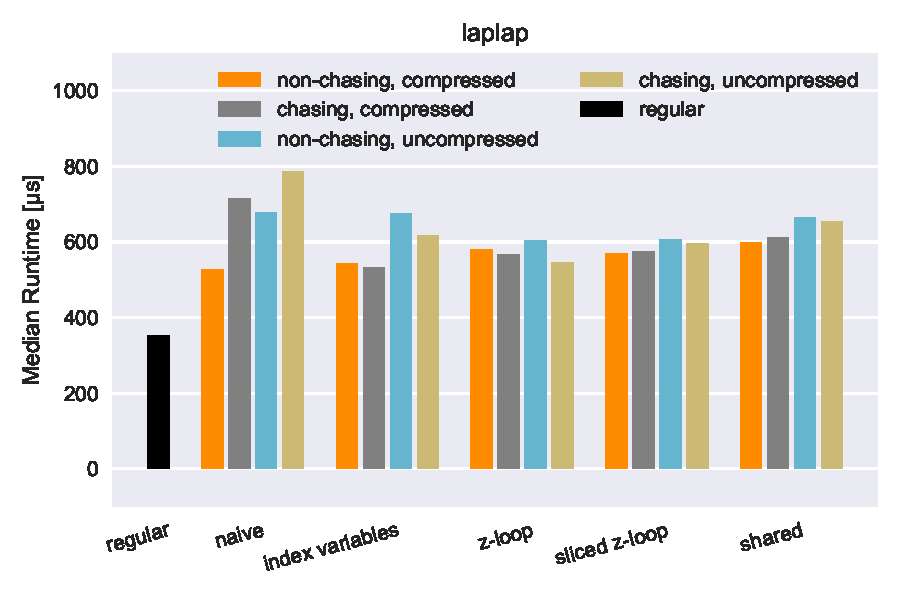
\includegraphics[scale=0.75]{laplap-zcurves-grouped-variants.pdf} % ./plot.py -i results/ultimate.csv -p grouped --size $((512*512*64)) --bar-groups variant --color storage --marker storage --z-curves z-curves --stencil laplap --title "laplap" -o results/variants/laplap-zcurves-grouped-variants.pdf --exclude laplap-regular-naive --scale-max 1000
	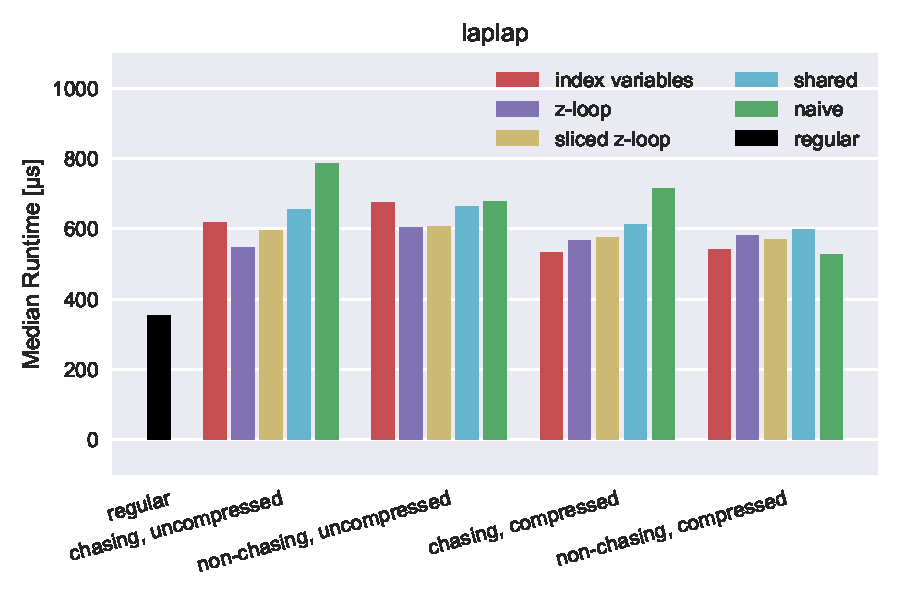
\includegraphics[scale=0.75]{laplap-zcurves-grouped-storage.pdf} % ./plot.py -i results/ultimate.csv -p grouped --size $((512*512*64)) --bar-groups storage --color variant --marker variant --z-curves z-curves --stencil laplap --title "laplap" -o results/variants/laplap-zcurves-grouped-storage.pdf --exclude laplap-regular-naive --scale-max 1000
	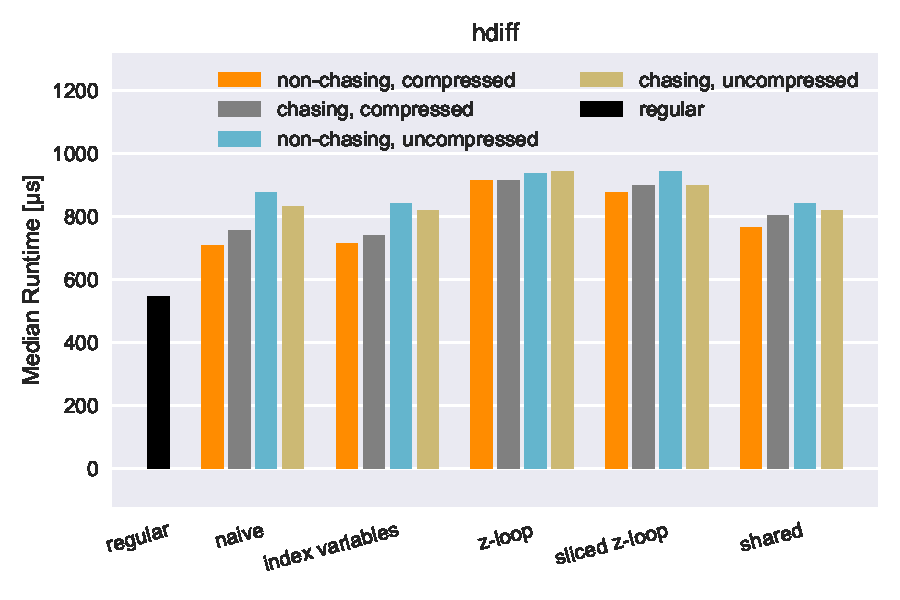
\includegraphics[scale=0.75]{hdiff-zcurves-grouped-variants.pdf} % ./plot.py -i results/ultimate.csv -p grouped --size $((512*512*64)) --bar-groups variant --color storage --marker storage --z-curves z-curves --stencil hdiff --title "hdiff" -o results/variants/hdiff-zcurves-grouped-variants.pdf --exclude hdiff-regular-naive --scale-max 1200
	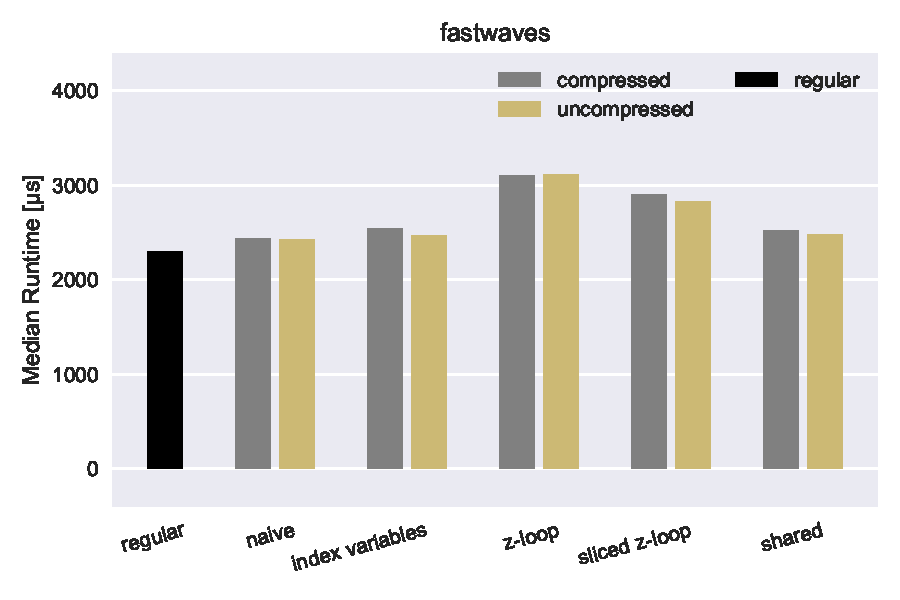
\includegraphics[scale=0.75]{fastwaves-zcurves-grouped-variants.pdf} % ./plot.py -i results/ultimate.csv -p grouped --size $((512*512*64)) --bar-groups variant --color storage --marker storage --z-curves z-curves --stencil fastwaves --title "fastwaves" -o results/variants/fastwaves-zcurves-grouped-variants.pdf --exclude fastwaves-regular-naive --scale-max 4000
	\caption{\label{fig:storage-access} Median runtimes across 20 runs for stencils on a $512\times512\times 64$-sized unstructured grid (z-curves layout). The fastest blocksize was chosen and reported per variant. The time reported for the regular grid is the fastest of all implemented regular variants. Results for row-major-stored grids are similar. Note that for the \emph{fastwaves} stencil, only direct neighbors are accessed; pointer chasing thus never occurs.}
\end{figure}

\subsubsection{\emph{Naive} and \emph{Idxvar} Access Strategies}
The \emph{naive} and \emph{idxvar} (index variables) access strategies are the fastest for all three stencils. In some cases, the \emph{naive} access strategy is faster than the \emph{idxvar} variant by a very slight margin. This is the case, for example, in the fastwaves stencil or the horizontal diffusion stencil executed on a non-chasing, compressed grid. This result might appear surprising at first, as the naive strategy repeatedly performs memory lookups for the same neighborship pointers. The index variables approach tries to reduce these reduntant lookups by storing the needed neighborship indices in temproary variables at the start of the kernel execution. However, this adds some overhead.

For one, the index variables variant for the fastwaves kernel leads to a higher register use when compiled (44 registers for \emph{idxvar} versus 42 for \emph{naive}). As registers are shared across threads of a block, this reduces the theoretical amount of threads that can be launched concurrently. As this difference is not present in the other stencils, this does not appear to be the main reason for the advantage, however. There are two more likely explanations for the advatnage of the \emph{naive} variant: First, access to the same memory location in the \emph{naive} kernel becomes as cheap as a register access after a neighborship pointer are read for the first time, as it will be held in the L1 cache. Reaccessing the same memory location helps keep the values fresh in all caches. As such, when a different thread requires the same memory location from the neighborship table, it is more likely to be in cache in the \emph{naive} variant. Second, the naive approach has better \emph{instruction level parallelism}. Because the index variables are assigned at the start of the \emph{idxvar} variant, all loads to the neighborship table are gathered in one sequence and must be executed before anything else. In the \emph{naive} approach, on the other hand, neighborship pointers are (re-)loaded only when needed in calculations. Thus, after one neighbor has been loaded, useful calculations using its value may already be performed. Table \ref{tab:fastwaves-naive-idxvar-metrics} details profiler metrics that support these claims.

\begin{table}
	\begin{tabular}{l l l}
		\hline
		Metric & \emph{naive} & \emph{idxvar} \\
		\hline
		Run time & $\mathbf{2438\mu s}$ & $2543\mu s$ \\
		Global load transactions & $126264460$ & $124235165$ \\
		L1 transactions & $38077396$ & $34593863$ \\
		L2 transactions & $56635611$ & $57264861$ \\
		Device Memory transactions & $36825619$ & $37327310$ \\
		Executed Instructions Per Cycle & $\textbf{0.522}$ & $0.497$ \\
		\hline
	\end{tabular}
	\caption{\label{tab:fastwaves-naive-idxvar-metrics}Selection of metrics for \emph{fastwaves} stencil run on a $512\times 512\times 1$-sized unstructured grid (z-curves layout, compressed neighborship table) with $32\times 1\times 8$ threads, which is the fastest block size for both variants. The \emph{naive} implementation is faster, even though it redoes the index lookups in the neighborship tables. The total global transaction count shows that the \emph{idxvar} variant successfully reduces the number of neighborship lookups performed. However, the cache transactions (L1 and L2) indicate that the naive variant keeps cache contents fresher and results in more cache hits. This is evidenced by the lower number of actual device memory reads in the naive approach, despite the idxvar approach requesting less memory.}
\end{table}

\subsubsection{\emph{Shared} Access Strategy}

% TODO
% - is almost same as idxvar due to caches
% - overhead of synchronization makes it slightly slower
% - back this up with metrics

\subsubsection{\emph{Z-loop} and \emph{Z-loop-sliced} Access Strategies}

% TODO
% - reiterate what the supposed advantage of z loop is
% - Why is it faster for uncompressed variants, why slower for compressed?
%    -> Back up with metrics!

\subsection{Effect of Problem Domain Size and Precision}

On grids of relatively large size ($512\times 512\times 64$), the fastest unstructured variants are between $5\%$ and $50\%$ slower than their regular counterparts, depending on the stencil. Generally, the relative slowdowns decrease with increasing domain size in the Z-dimension ($512\times 512\times 1$ up to $512\times 512\times 64$). This can be explained by the regularity of the grid in the Z-dimension, which some of the optimized implementations make use of. Theoretically, only one lookup to determine neighboring indices is required for all cells in a grid with equal X- and Y-coordinates. Even the unoptimized variants profit from this regularity, as neighborship information appears to be mostly kept in the caches.

For smaller grids ($128\times 128\times 64$), slowdowns are larger.

\begin{figure}
	\makebox[\textwidth]{
	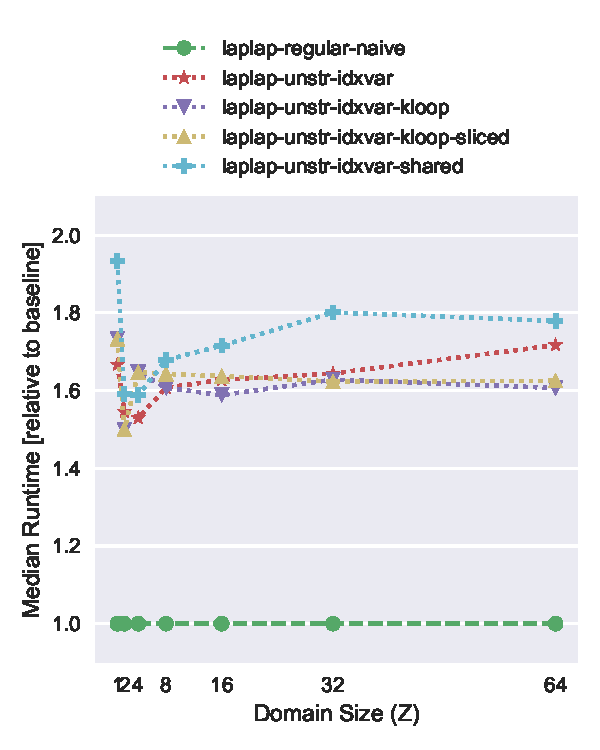
\includegraphics[width=0.3\paperwidth]{laplap-512x512-size-z.pdf}
	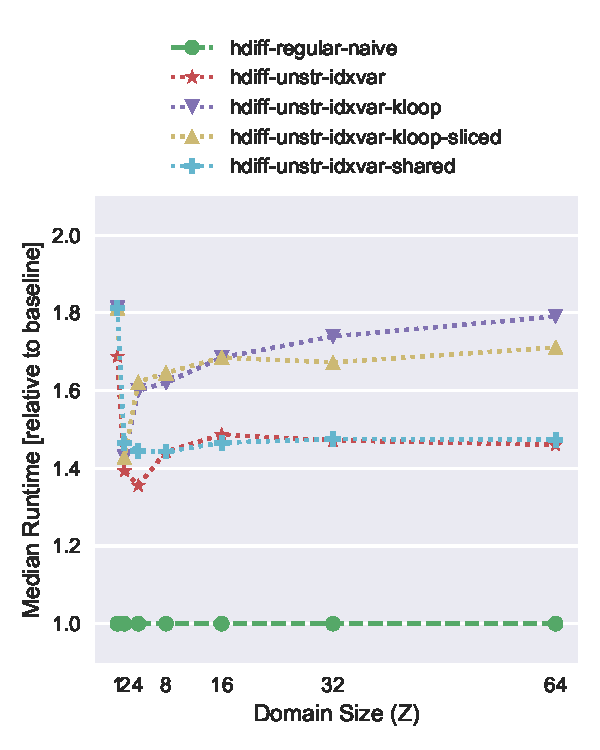
\includegraphics[width=0.3\paperwidth]{hdiff-512x512-size-z.pdf}
	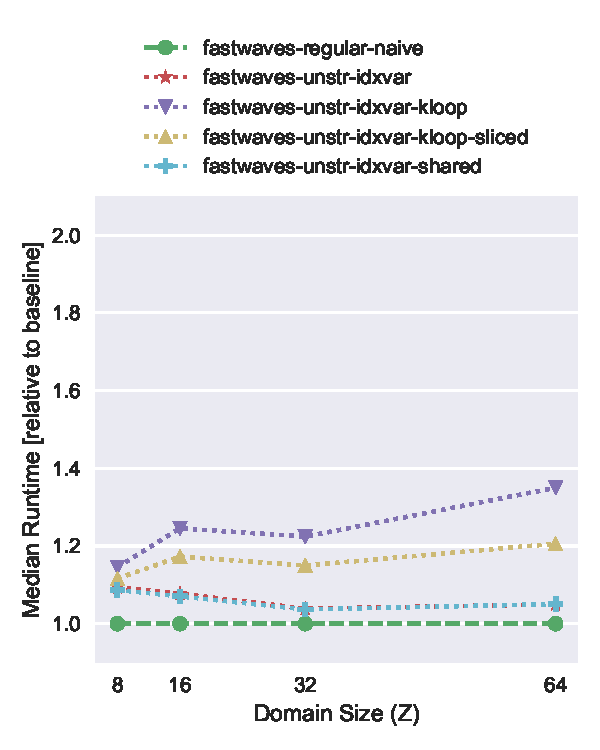
\includegraphics[width=0.3\paperwidth]{fastwaves-512x512-size-z.pdf}
	}
	\caption{\label{fig:results-512-sizes}Runtimes relative to stencil on regular grids sized $512\times 512\times 1$ up to $512\times 512\times 64$}
\end{figure}

% TODO
% - effect of Z-size increase
%   -> graph per variant (choose best-looking storage strategy if all similar)
%   -> reiterate how this shows that z regularity is made use of in certain variants
%   -> point to latency for first neighbor lookups that cannot be hidden
% - effect of XY-size change
%   -> smaller sizes 128x128x64
%   -> larger sizes 512x512x64
% - effect of precision
%   -> grouped bar graph double vs single; keep short

\subsection{Effect of stencil properties}

A major factor determining the relative cost of switching to an unstructured grid is the complexity of the original stencil. In stencils with fewer fields, such as the \emph{Laplace of Laplace} stencil, the additional lookups required in indirect adressing resulted in a larger relative cost. In the \emph{Fast Waves} stencil, which for its 9 fields requires many memory accesses already in its regular version, the overhead of indirect addressing is less noticeable in relation to the toal run time. 

% TODO
% - more fields -> less relative overhead; absolute? (might also decrease due to latency hiding with other field transactions)
% - more neighbors

\subsection{Optimal Block Size}

\subsubsection{Background}

One of the main determining factors for performance of a kernel is its launch configuration, which includes its grid size (number of blocks) and block size (number of threads, see section \ref{sec:hardware}). Cuda provides the option to specify block sizes in three dimensions, providing each thread with a X-, Y- and Z-index. In our benchmarks, we have tested all possible combinations of block sizes in steps of powers of two from 32 up to 512.

In order to cover the entire problem domain (which remains constant in size), a decrease in number of threads is always accompanied by an increase in the number of blocks (grid size), and vice versa. Owing to the way we map thread indices onto memory indices (X thread index maps onto memory index directly), thread sizes in the X-dimension of less than $32$ are highly inefficient. They lead to non-coalescing memory accesses. The X-dimension of the benchmarked block sizes is therefore always at least $32$.

\subsubsection{Overview}

The optimal \emph{total number} of threads depends mostly on the grid access implementation employed. In general, the same patterns can be observed for all three tested stencils and for all tested grid memory storage implementations: When using the \emph{naive}, \emph{idxvar} or \emph{shared} grid access strategies, it is best to have a high number of threads in total (256-512). The \emph{kloop} and \emph{kloop-sliced} thrive on a lower number of threads due to occupancy concerns. An exemplary overview of the runtimes as a function of total block size is given in figure \ref{fig:blocksizes-overview}.

\begin{figure}
	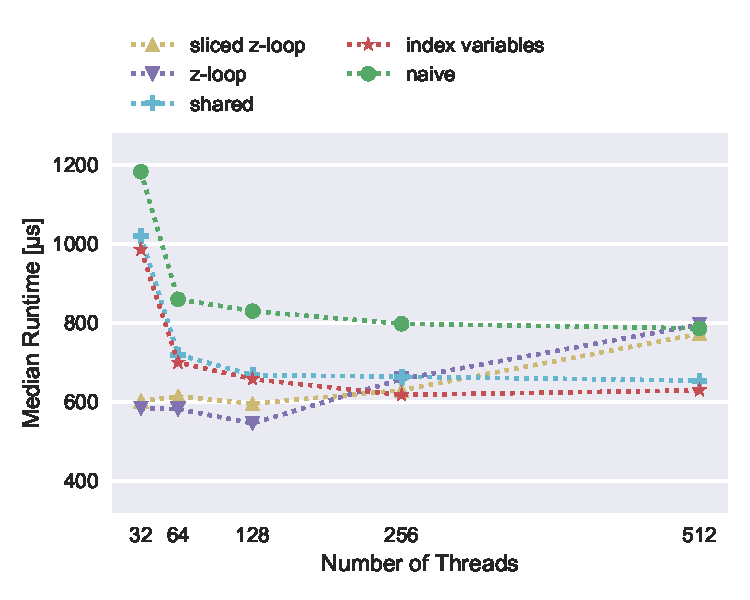
\includegraphics[scale=0.75]{laplap-z-curves-no-comp-chase-threads-prod.pdf}
	\caption{\label{fig:blocksizes-overview} Overview of the runtime for different implementations of the \emph{laplap} stencil on a $512\times 512\times 64$-sized domain (unstructured grid, pointer chasing, z-curves layout, uncompressed neighborship table) as a function on different total block sizes (product of X-, Y- and Z-blocksize). Results for other stencils and variants are of similar shape.}
	% ./plot.py -i results/ultimate.csv --size 16777216 -p line -x threads-prod --stencil laplap --z-curves z-curves --chase chase --comp no-comp  --marker variant --scale-min 400 --scale-max 1200 --plot-size 5 4
\end{figure}

The best \emph{shape} of the block size vector changes with the used grid storage strategy. Using \emph{uncompressed} neighborship tables, it is best for the \emph{naive}, \emph{idxvar} and \emph{shared} access strategies to have 32 or 64 threads in X-dimension and the rest in Z-dimension. Those implementations profit of more Z-threads because of the regularity of the grid in the Z-dimension. The \emph{non-chasing} variants profit even more of additional threads in the Z-dimension. This is due to the fact that in non-chasing variants, more neighborships are stored in the table; cache entries are thus evicted faster if many different X- and Y-coordinates are accessed. Switching to \emph{comepressed} neighborship tables, additional threads in the Z-dimension are of no use to any of the access strategies -- the reduced number of neighborship table entries after compression is accessed often enough to remain in cache independent of the Z-dimension of the block size. See figure \ref{fig:blocksizes-z} for a comparision of how changes in the Z-dimension of the blocksize vector translate to runtime changes. Whether the grid is stored as row-major or using z-order curves does not impact the required block sizes.

\begin{figure}
	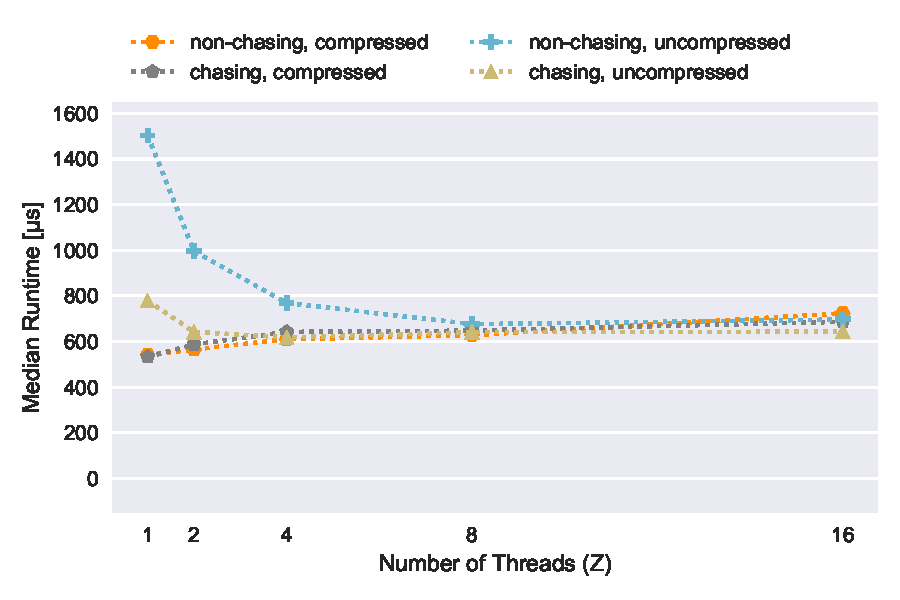
\includegraphics[scale=0.75]{laplap-zcurves-idxvar-threads-z.pdf} % ./plot.py -b unstr -i results/ultimate.csv --stencil laplap --variant idxvar --z-curves z-curves --size $((512*512*64)) --color storage --marker storage -p line -x threads-z -o results/blocksizes/laplap-zcurves-idxvar-threads-z.pdf --scale-max 1500
	\caption{\label{fig:blocksizes-z}Fastest runtimes for each fixed number of threads in the Z-dimension (other dimensions free) for the \emph{laplap} stencil on a $512\times 512\times 64$-sized domain (unstructured grid, row-major storage) for compressed and uncompressed variants, with and without pointer chasing.}
\end{figure}

\subsubsection{Optimal Block Sizes per Access Strategy}

\paragraph{\emph{Naive}, \emph{Idxvar} and \emph{Shared} Grid Access Strategies}
In order to always cover the entire problem domain, the number of blocks $b$ in each dimension in the \emph{naive}, \emph{idxvar} and \emph{shared} grid access strategies is chosen as a function on the problem size $d$ and the chosen number of threads $t$ as follows:
$$b = \begin{pmatrix}\left\lceil\frac{d_x}{t_x}\right\rceil & \left\lceil\frac{d_y}{t_y}\right\rceil & \left\lceil\frac{d_z}{t_z}\right\rceil\end{pmatrix}^\top$$

For the \emph{naive}, \emph{idxvar} and \emph{shared} implementations, a high number of threads per block is beneficial to performance. For grids using an uncompressed neighborship table, increasing the number of threads in the Z-dimension especially improves performance.

For the \emph{naive} and \emph{idxvar} strategies, the advantage of multiple threads in Z (in grids using uncompressed neighborship tables) can be explained through the regularity of the unstructured grid in Z-direction: Cells with identical X and Y coordinates share the same entry in the neighborship table. By having multiple threads in a block operate on different Z-levels, caching of this neighborship table entry becomes very effective. Evidence for this presumed reason for the speedup is given by two facts: One, of all block size combinations tested, the ones with more threads in the Z-dimension perform best. Two, the Nvidia profiler reports higher cache hit rates if the number of threads in Z-dimension is increased. As an example of this for the \emph{idxvar} access strategy, see table \ref{tab:laplap-blocksize-metrics}.

These effects are strongest for grids that also store neighbors-of-neighbors in the neighborship table (no pointer chasing). As this leads to a larger number of entries in the neighborship table that are stored and accessed, entries may be evicted from the cache more quickly. More threads in the Z-dimension, which access the same neighborship table entries, prevent this.

At the opposite end of the spectrum lie the grids stored using compressed neighborship tables. These tables are much smaller, and the same few entries are accessed in almost all threads. Because of this, neighborship table entries remain in cache no matter the shape of the block size vector, and additional threads in the Z-dimension bring no benefit. Cache locality for the accessed values is more important here; depending on the used layout for the values (z-order-curves or row-major) this means adding additional threads in X (z-curves, spatial locality given), or X and Y (row-major, adding another thread in Y gives some spatial locality).

\begin{table}
%	\begin{tabular}{l l l l l}
%		Blocksize & \texttt{global\_hit\_rate} & \texttt{tex\_cache\_hit\_rate} & \texttt{l2\_tex\_read\_hit\_rate} & \texttt{l2\_tex\_hit\_rate} \\
%		\hline
%		$32\times 1\times 1$ & $45.42\%$ & $44.39\%$ & $73.86\%$ & $67.69\%$ \\
%		$32\times 1\times 2$ & $58.83\%$ & $57.96\%$ & $76.60\%$ & $68.12\%$ \\
%		$64\times 1\times 2$ & $62.25\%$ & $66.21\%$ & $69.99\%$ & $60.36\%$ \\
%		$64\times 1\times 4$ & $72.33\%$ & $71.72\%$ & $72.77\%$ & $60.81\%$
%	\end{tabular}
	\begin{tabular}{l l l l l}
		Blocksize & \texttt{tex\_cache\_hit\_rate} & \texttt{l2\_tex\_hit\_rate} \\
		\hline
		$32\times 1\times 1$ & $44.39\%$ & $67.69\%$ \\
		$32\times 1\times 2$ & $57.96\%$ & $68.12\%$ \\
		$64\times 1\times 2$ & $66.21\%$ & $60.36\%$ \\
		$64\times 1\times 4$ & $71.72\%$ & $60.81\%$
	\end{tabular}
	\caption{\label{tab:laplap-blocksize-metrics} Cache hit rates for different block sizes for the \emph{laplap} stencil using a \emph{idxvar} grid access strategy on a $512\times 512\times 64$-sized domain (unstructured grid, pointer chasing, stored in z-curves layout, uncompressed neighborship table)}
\end{table}

By the design of the \emph{shared} access strategy, a speedup is supposed to be attained with a larger number of Z-threads; if there are more threads in Z-dimension within a block, more sharing of neighborship relations through shared memory can take place. These implementations indeed profit from more threads through shared memory in much the same way as \emph{naive} and \emph{idxvar} variants profit from more threads through the cache in the uncompressed grids.

\paragraph{\emph{Z-loop} and \emph{Z-loop-sliced} Grid Access Strategies}
Contrary to the other stencils, the \emph{z-loop} and \emph{z-loop-sliced} grid access strategies suffer from a high total thread count. As both of these strategies require one thread to perform calculations for multiple cells on different Z-levels, the total number of blocks and threads required to cover the entire grid is smaller. On the largest tested grid size ($512\times 512\times 64$), this leads to occupancy issues: As threads stall, there is not enough work can be scheduled to certain streaming multiprocessors to hide that latency. All threads inside a block are required to be executed on the same SM. Having more threads inside a block thus gives less blocks that can be scheduled onto stalled SMs. Smaller block sizes, on the other hand, give the scheduler a larger pool of blocks to choose from when trying to hide latency. Compare table \ref{tab:laplap-blocksize-occupancy} for an example of how a too large block size negatively impacts the \emph{kloop} implementation of the exemplary \emph{laplap} benchmark.

\begin{table}
	\begin{tabular}{l l l l l}
		Variant & Blocksize & Runtime & \texttt{achieved\_occupancy} & \texttt{issue\_slot\_utilization} \\
		\hline
		idxvar & $512$ & $783\mu s$ & $85\%$ & $19\%$ \\
		idxvar & $128$ & $844\mu s$ & $\mathbf{92\%}$ & $18\%$ \\
		idxvar & $32$  & $986\mu s$ & $48\%$ & $16\%$ \\
		z-loop & $512$ & $796\mu s$ & $25\%$ & $10\%$\\
		z-loop & $128$ & $\mathbf{546\mu s}$ & $42\%$ & $13\%$ \\ 
		z-loop & $32$  & $584\mu s$ & $41\%$ & $12\%$
	\end{tabular}
	\caption{\label{tab:laplap-blocksize-occupancy} Runtimes and occupancy metrics of \emph{idxvar} and \emph{z-loop} variant implementations of a \emph{laplap} stencil on an unstructured grid (size $512\times 512\times 64$, uncompressed neighborship table, z-curve memory layout, pointer chasing) for a selection of block sizes. The following block shapes were used: $512 = 256\times 2\times 1$, $128 = 64\times 2\times 1$ and $32 = 32\times 1 \times 1$. This highlights the occupancy issues the z-loop variant faces with too large block sizes. Note how the occupancy drops with increased number of threads for the z-loop variant, and how the runtime increases with it.}
\end{table}